\documentclass[review,
3p]{elsarticle} %review=doublespace preprint=single 5p=2 column
%%% Begin My package additions %%%%%%%%%%%%%%%%%%%

\usepackage[hyphens]{url}

  \journal{Malaria Journal} % Sets Journal name

\usepackage{lineno} % add

\usepackage{graphicx}
%%%%%%%%%%%%%%%% end my additions to header

\usepackage[T1]{fontenc}
\usepackage{lmodern}
\usepackage{amssymb,amsmath}
\usepackage{ifxetex,ifluatex}
\usepackage{fixltx2e} % provides \textsubscript
% use upquote if available, for straight quotes in verbatim environments
\IfFileExists{upquote.sty}{\usepackage{upquote}}{}
\ifnum 0\ifxetex 1\fi\ifluatex 1\fi=0 % if pdftex
  \usepackage[utf8]{inputenc}
\else % if luatex or xelatex
  \usepackage{fontspec}
  \ifxetex
    \usepackage{xltxtra,xunicode}
  \fi
  \defaultfontfeatures{Mapping=tex-text,Scale=MatchLowercase}
  \newcommand{\euro}{€}
\fi
% use microtype if available
\IfFileExists{microtype.sty}{\usepackage{microtype}}{}
\usepackage[]{natbib}
\bibliographystyle{model6-num-names}

\ifxetex
  \usepackage[setpagesize=false, % page size defined by xetex
              unicode=false, % unicode breaks when used with xetex
              xetex]{hyperref}
\else
  \usepackage[unicode=true]{hyperref}
\fi
\hypersetup{breaklinks=true,
            bookmarks=true,
            pdfauthor={},
            pdftitle={Reported reasons for non-use of insecticide-treated nets in large national household surveys},
            colorlinks=false,
            urlcolor=blue,
            linkcolor=magenta,
            pdfborder={0 0 0}}

\setcounter{secnumdepth}{5}
% Pandoc toggle for numbering sections (defaults to be off)


% tightlist command for lists without linebreak
\providecommand{\tightlist}{%
  \setlength{\itemsep}{0pt}\setlength{\parskip}{0pt}}

% From pandoc table feature
\usepackage{longtable,booktabs,array}
\usepackage{calc} % for calculating minipage widths
% Correct order of tables after \paragraph or \subparagraph
\usepackage{etoolbox}
\makeatletter
\patchcmd\longtable{\par}{\if@noskipsec\mbox{}\fi\par}{}{}
\makeatother
% Allow footnotes in longtable head/foot
\IfFileExists{footnotehyper.sty}{\usepackage{footnotehyper}}{\usepackage{footnote}}
\makesavenoteenv{longtable}

% Pandoc citation processing
\newlength{\cslhangindent}
\setlength{\cslhangindent}{1.5em}
\newlength{\csllabelwidth}
\setlength{\csllabelwidth}{3em}
\newlength{\cslentryspacingunit} % times entry-spacing
\setlength{\cslentryspacingunit}{\parskip}
% for Pandoc 2.8 to 2.10.1
\newenvironment{cslreferences}%
  {}%
  {\par}
% For Pandoc 2.11+
\newenvironment{CSLReferences}[2] % #1 hanging-ident, #2 entry spacing
 {% don't indent paragraphs
  \setlength{\parindent}{0pt}
  % turn on hanging indent if param 1 is 1
  \ifodd #1
  \let\oldpar\par
  \def\par{\hangindent=\cslhangindent\oldpar}
  \fi
  % set entry spacing
  \setlength{\parskip}{#2\cslentryspacingunit}
 }%
 {}
\usepackage{calc}
\newcommand{\CSLBlock}[1]{#1\hfill\break}
\newcommand{\CSLLeftMargin}[1]{\parbox[t]{\csllabelwidth}{#1}}
\newcommand{\CSLRightInline}[1]{\parbox[t]{\linewidth - \csllabelwidth}{#1}\break}
\newcommand{\CSLIndent}[1]{\hspace{\cslhangindent}#1}

\usepackage{floatrow}
\floatsetup[figure]{capposition=top}
\floatplacement{figure}{H}
\usepackage{setspace}\doublespacing
\biboptions{sort&compress}
\usepackage{booktabs}
\usepackage{longtable}
\usepackage{array}
\usepackage{multirow}
\usepackage{wrapfig}
\usepackage{float}
\usepackage{colortbl}
\usepackage{pdflscape}
\usepackage{tabu}
\usepackage{threeparttable}
\usepackage{threeparttablex}
\usepackage[normalem]{ulem}
\usepackage{makecell}
\usepackage{xcolor}



\begin{document}


\begin{frontmatter}

  \title{Reported reasons for non-use of insecticide-treated nets in
large national household surveys}
    \author[Tropical Health LLP]{Hannah Koenker}
   \ead{hannah@trophealth.com} 
    \author[International Federation of the Red Cross and Red Crescent
Societies]{Marcy Erskine}
   \ead{marcy.erskine@ifrc.org} 
    \author[International Federation of the Red Cross and Red Crescent
Societies]{Robert Opoku}
   \ead{robert.opoku@ifrc.org} 
    \author[International Federation of the Red Cross and Red Crescent
Societies]{Zainab Ali}
   \ead{zainab.ali@ifrc.org} 
    \author[Tropical Health LLP]{Eleanore Sternberg}
   \ead{eleanore@trophealth.com} 
    \author[ICF]{Cameron Taylor}
   \ead{cameron.taylor@icf.com} 
      \affiliation[Tropical Health LLP]{Baltimore, USA}
    \cortext[cor1]{Corresponding author}
  
  \begin{abstract}
  Insecticide-treated nets (ITN) are the cornerstone of modern malaria
  vector control, with over 2 billion ITNs delivered to households in
  endemic areas since 2000. ITN access, i.e.~availability within the
  household, based on the number of ITNs and number of household
  members, is the sine qua non of ITN use. Once ITNs are in a given
  household, however, individuals may choose to use or not use them on a
  given night, with structural, cultural, opportunistic, and social
  barriers impeding optimal use. Factors determining ITN use are
  frequently examined in published literature, but to date, large
  household survey data on reasons given for non-use of nets have not
  been explored.

  A total of 155 DHS, MIS, and MICS surveys since 2003 were downloaded
  with permission and reviewed for presence of questions on reasons why
  nets were not used the previous night, and twenty-four surveys were
  identified. The percent of nets that were reported used the previous
  night was calculated for 155 surveys, and frequencies and proportions
  of reasons for non-use were calculated within the twenty-four surveys.
  Results were stratified by household supply of ITNs in three
  categories (not enough'', ``enough'', and ``more than enough'').

  The percent of nets used the previous night averaged 70.4\% across the
  155 surveys conducted since 2003. Stratifying by households ITN
  supply, this was 75\%, 71\%, and 53\% for households with not enough,
  enough, and more than enough ITNs, respectively. Population ITN use
  within these households was 51\%, 74\%, and 76\%, respectively.
  Reported reasons for non-use of ITNs were primarily nets being extra
  or being saved for later, followed by low perceived risk of malaria
  (no mosquitoes/no malaria). The least frequent categories cited as
  reasons for nets not being used were ``net attributes'' (size, shape,
  color, etc) and ``fears''. Using continuous DHS data from Senegal, the
  proportions of nets used peaked during high transmission season, while
  ``no/few mosquitoes'' responses peaked during the dry season.

  The proportion of nets used the previous night has averaged over 70\%
  since 2003, with no discernible change over this period. Reported
  reasons for why a net goes unused fall largely into three categories -
  nets that are extra/being saved for future use; the perception that
  there is little risk of malaria (particularly in dry season); and
  ``other'' responses. Net attributes such as color, size, shape, and
  texture, and fears related to chemicals were the least frequent
  reasons given. Classifying reasons for non-use into broader categories
  facilitates the design of appropriate social and behaviour change
  interventions to address the major underlying reasons for non-use,
  where this is feasible. Finally, national malaria programs should
  request the inclusion of this question in future surveys to provide
  actionable data to inform SBC programming. {[}Meant to be 350 words
  max; it's over currently{]}
  \end{abstract}
    \begin{keyword}
    insecticide-treated nets \sep long-lasting insecticidal nets \sep 
    net use
  \end{keyword}
  
 \end{frontmatter}

\hypertarget{introduction}{%
\section{Introduction}\label{introduction}}

Insecticide-treated nets (ITN) are the cornerstone of modern malaria
vector control, with over 2 billion ITNs delivered to households in
endemic areas since 2000 \citep{Milliner:2016um}. Consistent use of ITNs
provides the most protection from malaria vectors, but households may
only have enough nets for all household members for the several months
immediately following mass ITN distributions, as nets begin to wear out
\citep{Bhatt:2015gn, Koenker:2018gx, Girond:2018bc, 10.1038/s41467-021-23707-7}.
ITN access, i.e.~availability within the household, based on the number
of ITNs and number of household members, is the sine qua non of ITN use.
Once ITNs are in a given household, however, individuals may choose to
use or not use them on a given night, with structural, cultural,
opportunistic, and social barriers impeding optimal use
\citep{Pulford:2011dc, 10.1080/13648470.2021.1884185}.

Many papers evaluate determinants of ITN use, although not all control
for ITN access. Primary factors influencing use of available nets
include perception of risk of malaria, due to seasonality of
transmission - ITN use among those with access is typically lower during
long, hot, dry seasons, when malaria vectors and other nuisance biting
insects are less abundant \citep{Koenker:2019id}. Perceptions of heat
and feeling closed in are frequently cited alongside each other
\citep{Pulford:2011dc, Ahorlu:2019ck}. ITN use is also affected by who
within a given household can share a single ITN, as well as space
available to hang ITNs
\citep{Toe:2009gb, Lam:2014fc, Galvin:2011ea, 10.1186/s12936-021-03705-2}.
The condition of an ITN, related to its age along with the development
of holes and tears, is associated with early discarding of ITNs and
therefore lack of use
\citep{10.1186/s12936-022-04126-5, 10.1371/journal.pmed.1003248, 10.1186/s12936-021-03686-2, 10.1186/s12936-021-03976-9};
the decay rate of ITNs is a critical component of overall trends in ITN
access, determining how quickly coverage declines following mass
distribution campaigns and other large-scale distributions
\citep{Bhatt:2015gn, 10.1038/s41467-021-23707-7}.

Pulford et al \citep{Pulford:2011dc} reviewed 22 available studies in
2011 for reasons why nets went unused, finding that discomfort due to
heat and perceived low risk of malaria due to low mosquito density were
the primary reasons cited, but noted that findings were tentative given
the dearth of published studies. Since this time, large national
household surveys including Malaria Indicator Surveys and Demographic
and Health Surveys have in several cases added questions about reasons
for not using nets. This paper summarizes available data in these MIS
and DHS surveys and explores trends in the percentage of ITNs used.
Finally, recommendations are given for further exploration of reasons
for non-use of ITNs.

\hypertarget{study-objectives}{%
\subsection{Study objectives}\label{study-objectives}}

The study objectives are to use national population-based household
survey data characterize reasons underlying non-use of ITNs. The goal of
the analysis is to explore the reasons for not using an ITN during the
previous night in relation to net supply at household level, and how
these reasons vary over time (where possible) and by country. The
primary research questions are:

\begin{enumerate}
\def\labelenumi{\arabic{enumi}.}
\tightlist
\item
  What proportion of nets were used the night prior to the survey?
\item
  Of nets that went unused, what are the primary reported reasons for
  non-use, and how do reasons vary by country and net supply?
\end{enumerate}

\hypertarget{methods}{%
\section{Methods}\label{methods}}

For the first study objective, 155 DHS, MIS, and MICS surveys since 2003
were downloaded with permission from dhsprogram.com and mics.unicef.org.
Each dataset was reshaped to a long format to create a net file that
included whether the net was observed by the interviewer, its age,
whether it was an ITN, the number of users, and whether it was reported
to have been used the previous night. The Roll Back Malaria indicator of
percent of nets used the previous night was calculated for all surveys
and linear regression used to assess temporal changes for each type of
survey. To evaluate net use in the context of household ITN supply, a
variable was computed with supply levels where ``not enough'' indicated
less than 0.5 nets available per person (\textless1 ITN per 2 people),
``enough'' indicated 0.5 to 0.75 nets available per person (≥1 ITN per 2
people), and ``more than enough'' nets indicated a supply of 0.75 or
more nets available per person (i.e.~at least 2 nets per 3 people).
Households consisting of one person with one net were categorized as
`enough', rather than ``more than enough''. For this variable, both
untreated nets and ITNs were included.

For the second study objective, all DHS and MIS surveys were reviewed
and twenty-four surveys from nine countries were identified as having
included a follow-up question for unused nets about why they were not
used. All were Malaria Indicator Surveys, conducted during peak malaria
transmission season, with the exception of the Madagascar 2021 DHS,
Nigeria 2018 DHS, the Tanzania 2015-16 DHS/MIS, and eight continuous DHS
surveys from Senegal (2011-2019), where fieldwork is conducted
throughout the year. Nets that were not observed by the interviewer were
excluded from analysis. The ``svy'' family of commands in Stata 17 was
used to appropriately weight results within each country. Plots were
produced with R.

\hypertarget{results}{%
\section{Results}\label{results}}

The percent of nets used the previous night averaged 70.4\% across all
available (n=155) DHS, MIS, and MICS surveys since 2003 (Fig.
\ref{fig_netsused}). Linear regression stratified by survey type
indicates that there was no significant change over time in the
percentage of nets used the previous night for MIS (p=0.772), DHS
(p=0.499) or MICS (p=0.235). MIS surveys, conducted during high
transmission season, were associated with a 6.8-point increase in rates
of net use when compared to DHS surveys (p=0.046), which are generally
conducted during dry season when malaria transmission is lower. Net use
rates in MICS surveys did not differ significantly from DHS surveys
(0.872).

\begin{figure}

{\centering 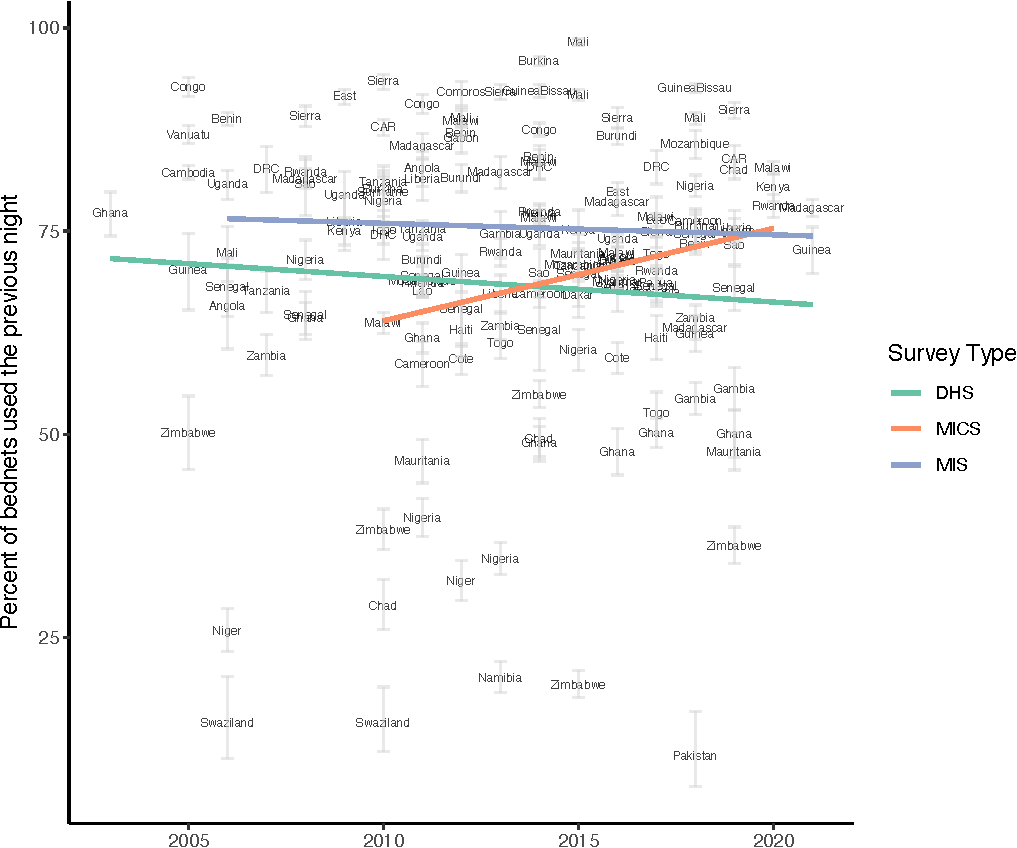
\includegraphics[width=0.8\linewidth]{reasons_paper_files/figure-latex/fig_netsused-1} 

}

\caption{\label{fig_netsused}Percentage of nets used the night before, DHS, MICS, MIS surveys 2003-2020}\label{fig:fig_netsused}
\end{figure}

The percent of nets used the previous night was 75\% for households with
not enough nets (at least one, but less than 1 net for 2 people) and
71\% for households with at least 1 net for 2 people but less than 2
nets for 3 people (net:person ratio between 0.5 and 0.75), shown in Fig.
\ref{fig_violin}. In contrast, in households with at least 2 nets for 3
people 53.2\% of nets were used, potentially reflecting excess nets
within the household or different net use behaviours by households with
excess nets. Nonetheless, in these same households with ``more than
enough'' nets, the percent of individuals using an ITN the previous
night was 76\%, on par with those living in households with sufficient
ITNs (73.5\%). For people living within households owning at least one
but not enough ITNs, population ITN use was 51.2\%.

\begin{figure}

{\centering 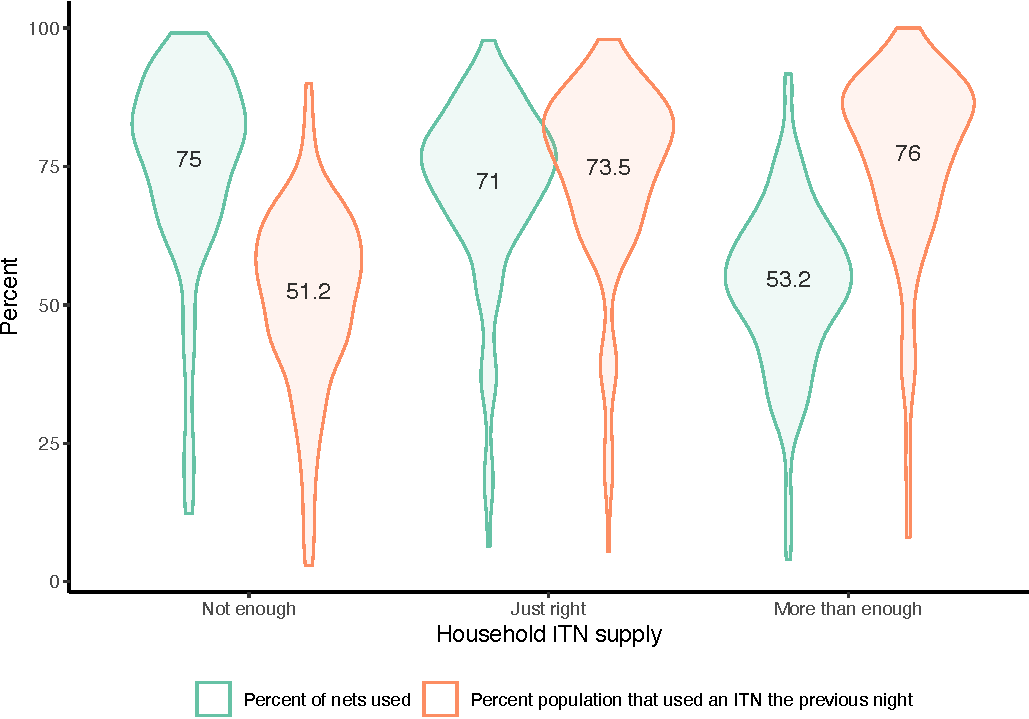
\includegraphics[width=0.8\linewidth]{reasons_paper_files/figure-latex/fig_violin-1} 

}

\caption{\label{fig_violin}Violin plots with means for ITNs used the previous night and population use of ITNs, by household net supply level.}\label{fig:fig_violin}
\end{figure}

\hypertarget{reported-reasons-for-not-using-nets}{%
\subsection{Reported reasons for not using
nets}\label{reported-reasons-for-not-using-nets}}

Response options for reasons why a net was not used the previous night
were inconsistent between countries and sometimes changed over time
within a given country. Table 1 summarizes the response options for the
question ``Why was this net not used the previous night?'' and
categorizes them into seven broad categories: `extra' (nets being saved
for later, or extra), `fears' (chemicals are unsafe or toxic), `net
attributes' (size, shape, or textile), `objective' (usual user not here;
net being washed; no space to hang; net too torn), `risk perception' (no
mosquitoes or no malaria), `subjective' (related to heat, smell, etc),
and `other' (capturing `other' as well as `not hung' and `net not needed
last night', all of which fail to provide useful information about the
respondent's reasoning). Risk perception and subjective reasons for a
net going unused may be more amenable to certain social behaviour change
interventions, while objective reasons are not. In eight surveys,
multiple responses were possible, while in sixteen, only a single
response could be selected.

\begin{longtable}[]{@{}
  >{\raggedright\arraybackslash}p{(\columnwidth - 2\tabcolsep) * \real{0.1871}}
  >{\raggedright\arraybackslash}p{(\columnwidth - 2\tabcolsep) * \real{0.8129}}@{}}
\caption{Categorization of reasons why nets were not
used}\tabularnewline
\toprule
\begin{minipage}[b]{\linewidth}\raggedright
Category
\end{minipage} & \begin{minipage}[b]{\linewidth}\raggedright
Answer options from MIS
\end{minipage} \\
\midrule
\endfirsthead
\toprule
\begin{minipage}[b]{\linewidth}\raggedright
Category
\end{minipage} & \begin{minipage}[b]{\linewidth}\raggedright
Answer options from MIS
\end{minipage} \\
\midrule
\endhead
extra & extra; saving for later; stored away \\
fears & chemicals not safe; net is bad for health;
superstition/witchcraft \\
net attributes & too rough/hard; too small; don't like color/shape/size;
brought bedbugs; prefer other method \\
objective & too old/torn/dirty; no place to hang; usual user didn't
sleep here; net being washed; too weak/difficult to hang \\
risk perception & no mosquitoes; no malaria; saving for rainy season; \\
subjective & too hot; don't like smell; feel closed in/afraid; no longer
kills/repels mosquitoes; child doesn't like; net never used; causes
itching/coughing; slept outdoors \\
other & not needed last night; not hung; other; don't know \\
\bottomrule
\end{longtable}

Figure \ref{summ_reas_cat} below shows the proportion of nets used the
previous night across twenty-four surveys in nine countries, and the
reasons why certain nets were not used. The percentage of nets reported
used ranged from 50\% in Ghana 2019 to 85\% in Mozambique 2018.
Senegal's continuous DHS surveys showed the highest proportions of
reasons related to risk perception, with up to 25\% of nets going unused
due to ``no mosquitoes'' or ``no malaria''. However, this category was
relatively infrequent in other surveys, with the exception of Tanzania
where up to 11\% of nets were unused due to risk perception, and was
more pronounced in lower-transmission areas (Supplemental Material).
``Extra/saving for later'' nets were reported most frequently in Ghana
2019 (19\%), Liberia 2016 (19\%), and in Tanzania (12-14\% of nets).
Senegal and Uganda had the highest rates of `other' responses. In 2018,
Uganda updated answer options for this question to be more detailed,
resulting in the `extra' and `objective' categories becoming more
prominent; `extra' category was comprised largely of `saving to replace
other net', while `objective' was a combination of `usual user not here'
and `too old/torn' (Supplemental Material). Subsequent surveys (Ghana,
Guinea, Mozambique, Madagascar) adopted similar answer options.

\begin{figure}

{\centering 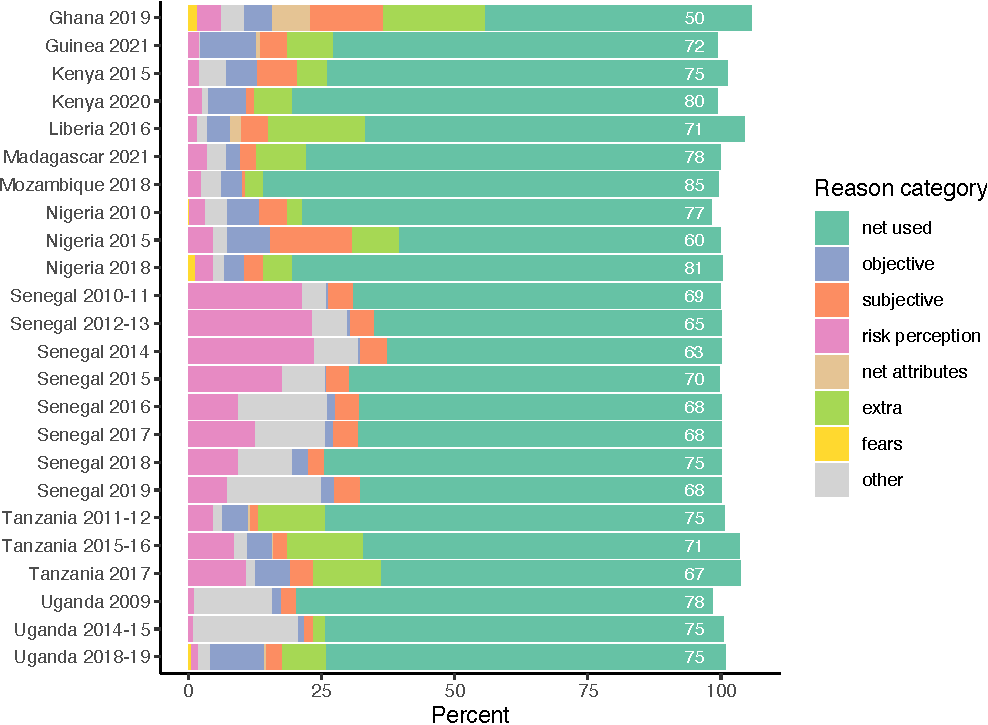
\includegraphics[width=0.8\linewidth]{reasons_paper_files/figure-latex/summ_reas_cat-1} 

}

\caption{\label{summ_reas_cat}Summary of reasons nets were not used, across surveys}\label{fig:summ_reas_cat}
\end{figure}

Figure \ref{fig_cats}A summarizes the categories of reasons for non-use
across the twenty-four surveys, demonstrating that an average of 71.5\%
of nets were used, and that the leading category for non-use was
``extra'', followed by ``risk perception''. The least frequent
categories cited as reasons for nets not being used were ``net
attributes'' and ``fears''. Figure \ref{fig_cats}B presents reasons for
nets not being used in the context of household net supply.

\begin{figure}

{\centering 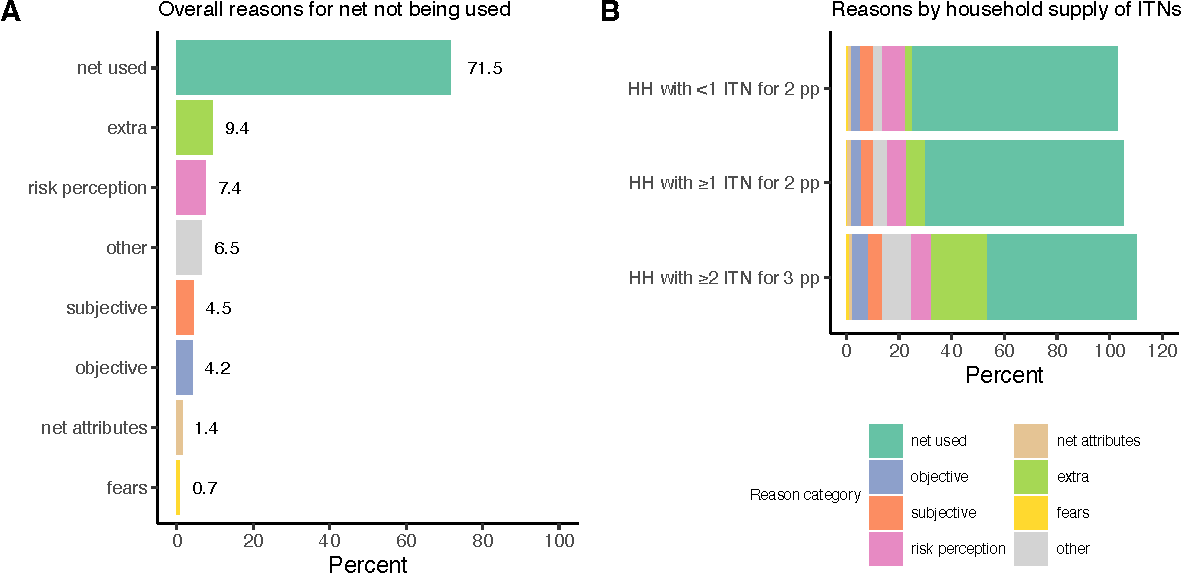
\includegraphics[width=1\linewidth]{reasons_paper_files/figure-latex/fig_cats-1} 

}

\caption{\label{fig_cats}Summary of reasons across surveys, by household supply of ITNs}\label{fig:fig_cats}
\end{figure}

Not surprisingly, ``extra'' nets comprised a higher proportion of
reasons for non-use among households with at least 2 ITN for 3 people
(21.6\%) compared to households with not enough nets (3\%) or households
with at least 1 ITN for 2 people (7.7\%). ``Other'' responses were more
frequent in households with at least 2 ITNs for 3 people (11.4\% vs
5.7\% and 3.9\%), indicating that `other' reasons are likely related to
having extra nets, particularly in surveys prior to 2018 when response
options did not capture extra nets well. The ``risk perception''
category was stable across ITN supply categories, ranging between 6.8\%
and 8.4\%, as were ``subjective'' reasons, ranging from 4.2\% to 5\%.
Reasons for non-use related to net attributes or fears comprised less
than 2\% across all ITN supply categories.

In each of the eight surveys from Senegal two questions were asked.
First, in households that owned at least one net, respondents were asked
``do members of this household use nets all year round'' (\ref{fig_sen}A
below). The proportion of respondents reporting people in their
household do use nets year-round increased from 47.4\% to 72.9\% over
the 2008-2019 period (p\textless0.001 for trend) and generally tracked
with increasing levels of population access to ITNs. Next, for
households responding ``no'', a follow-up question was asked: ``what are
the reasons household members do not use nets year round?''. The most
frequent answer was ``no/few mosquitoes'' (\ref{fig_sen}B), which fell
from a high of 29.1\% in 2012 to 14.5\% in 2019, as a proportion of all
households in the survey. ``Heat'' was the next most common response,
ranging between 2.1-4.9\%. Not liking the net and forgetfulness were
relatively uncommon (less than 2.6\% and 1.2\% of all households in any
survey, respectively).

\begin{figure}

{\centering 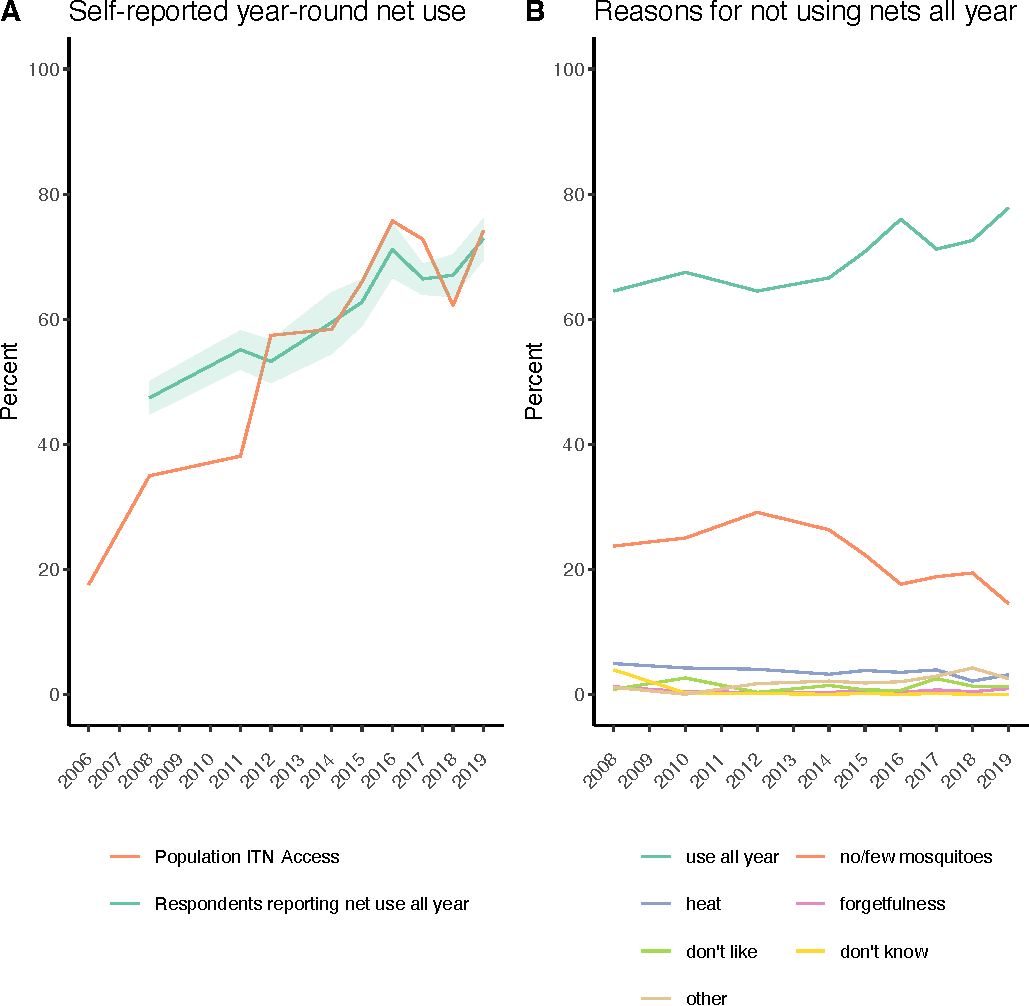
\includegraphics[width=0.8\linewidth]{reasons_paper_files/figure-latex/fig_sen-1} 

}

\caption{\label{fig_sen}Year-round net use and reasons for not using nets, Senegal 2008-2019}\label{fig:fig_sen}
\end{figure}

\begin{figure}

{\centering 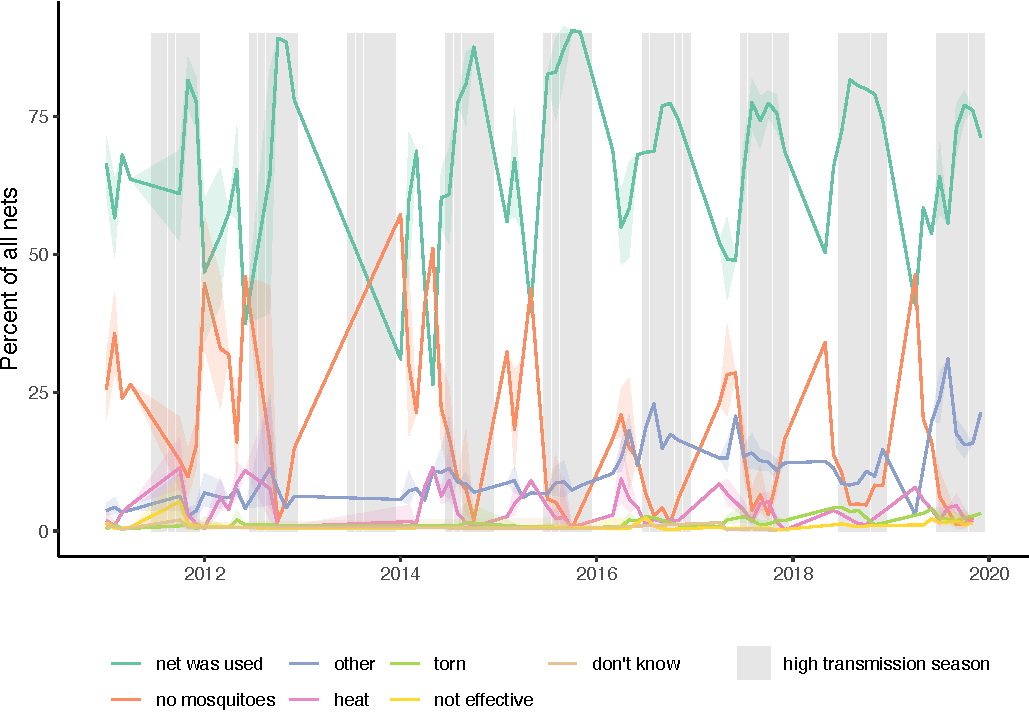
\includegraphics[width=0.8\linewidth]{reasons_paper_files/figure-latex/seasons_fig-1} 

}

\caption{\label{seasons_fig}Reported net use and reasons for non-use, Senegal 2011-2019}\label{fig:seasons_fig}
\end{figure}

Seasonal trends in reasons for not using nets in Senegal were apparent,
as illustrated in Fig. \ref{seasons_fig} above. The percentage of nets
used the previous night peaked during high transmission season (shown
approximatively above as July-December), falling to lower levels during
the drier months of February-May. Correspondingly, the proportion of
nets not used due to ``no mosquitoes'' peaked during the drier months.

\hypertarget{discussion}{%
\section{Discussion}\label{discussion}}

Over the past nearly twenty years, an average of over 70\% of ITNs were
reported used the previous night in large household surveys. Questions
about why nets go unused have only been included in twenty-four surveys
from nine countries, but among these, the primary reasons given are that
unused nets are surplus to immediate requirements, or not needed due to
perceived low risk of malaria and/or mosquito bites. Responses related
to extra nets were more frequent among households owning more ITNs than
strictly deemed necessary by WHO (1 ITN per 2 people)
\citep{WorldHealthOrganization:2019ws}. Unsurprisingly, the proportion
of nets used the previous night in households with ``more than enough''
nets was lower than for households with less than enough or ``enough''
nets, while at the same time, the proportion of people that used an ITN
the previous night was highest in households with ``enough'' or ``more
than enough'' ITNs. Households with more than one ITN per two people may
have acquired additional nets to cover individual sleeping spaces or to
accommodate sleepers who cannot share a sleeping space; other households
may have extra nets being saved for later use, when current nets wear
out, and thus are able to have most household members sleep under one.
Households with ``not enough'' ITNs had lower rates of population use,
but high rates of nets being used - indicating that these households are
using the nets they have, and are challenged primarily by not having
enough for other members of the family. It should be noted that having
`extra' nets is reflective of the inherent inefficiencies of ITN
distribution systems, wherein some households will have too few while
others may receive additional nets slightly earlier than required
\citep{Bhatt:2015gn}. The authors view having extra nets on hand within
households as a positive, given the unpredictability of net replacement
timing.

Reasons related to net attributes - including size, shape, color,
texture, and mosquito-killing ability - were inconsistently included in
survey questionnaires, but represented a negligible fraction of reasons
for not using nets. While this does not preclude these issues from
contributing to net non-use, it provides some evidence that these issues
are not top of mind when families are making net use decisions. The 2011
Pulford review findings \citep{Pulford:2011dc} that discomfort due to
heat and perceived low mosquito density were the most widely identified
reasons for non-use are partially confirmed here; heat per se was not
widely reported in more recent surveys, but risk perception as a
category, particularly for Senegal, was a key driver. Pulford et al also
use categories such as ``social factors'' (sleeping elsewhere),
``technical factors'' (not being able to hang a net), which are
considered ``objective'' reasons for non-use in our study. Pulford's
review, conducted just as universal coverage campaigns were scaling up,
was limited to 22 studies between 1990 and 2010. Since this time, a
number of qualitative research studies have also been conducted, in
which respondents cite being bothered by net attributes including smell,
itching, shape, and size
\citep{Mattern:2016dp, Berthe:2014ja, Sande:2012vb, Galvin:2011ea}.
However, these reasons are only rarely cited during quantitative surveys
included in this study. Research from Senegal indicates that initial
itching or smell are transitory, noticeable when nets are first
received, but subsiding over time, not impeding net use
\citep{Berthe:2014ja}. Other less preferable attributes of nets may
similarly be less noticeable over time, and are no longer a key reason
for non-use, particularly when, as in most countries distributing ITNs,
there are seldom enough nets in good condition for everyone to use.
Families are thus obliged to use the imperfect ITNs they have, or risk
contracting malaria.

Nearly 80 unique answer options were included across the surveys. The
categorization of responses into ``extra'', ``risk perception'',
``objective'', ``subjective'', etc., is intended to facilitate
interpretation and guide national malaria programmes and their partners
in designing appropriate responses for improving net use. Where the
majority of unused nets are not used due to subjective reasons, social
behaviour change may be able to change attitudes and behaviours;
however, if most nets are unused due to being too old or torn,
programmes may need to focus on net maintenance behaviours and/or
additional ITN distribution to improve ITN use rates.

As one example, Senegal has focused messaging over the last decade to
address the perceived lower risk of malaria in the hot/dry season, in
part because of findings in these surveys, through the ``Trois Toutes''
campaign (``Toute la famille, toutes les nuits, toute l'année'' or
``Every family member; every night; all year round''). Self-reported use
of nets all year round has increased over time, although it remains
unclear whether this is driven primarily by corresponding increases in
overall access to ITNs with the household, or represent real changes in
behaviour for more consistent ITN use. The continuous DHS in Senegal,
conducted annually for the last eight years over multiple months,
present a unique opportunity for assessing trends over time in
year-round use as well as evaluating the associations between seasons
and frequency of certain responses, notably ``no/few mosquitoes''.
Indeed, net use peaks in high transmission season, while the proportion
of nets not used due to ``no mosquitoes'' peaks during the hot dry
season when mosquito densities are substantially lower.

Another example of refining this question to better inform programming
is Uganda. Following the 2009 survey Uganda implemented ``hang up
campaigns'' to ensure nets were hung and used, partially in response to
low hanging rates observed in the 2009 and other surveys. Operational
research showed that these hang-up campaigns did not improve hanging or
use rates, as net hanging increased at similar rates over time in
control and intervention groups \citep{Anonymous:2015ff}. In its most
recent surveys, Uganda teased apart the nebulous ``not hung'' answer
option to better focus on specific barriers to net use, enabling the
programme to understand what lies behind the non-use of nets; key
reasons for non-use in 2018 were ``saving net for later'', ``user not
here'', and ``too old/torn'', none of which are best addressed with SBC
efforts to hang up nets. This pragmatic specification of reasons for
non-use enables programmes and their SBC partners to better design and
target net use interventions. However, the absence of these types of
questions even in many recent surveys is a missed opportunity,
particularly as ITNs remain the primary tool for malaria vector control
across the globe. National malaria programmes would do well to ensure
this question is included in their upcoming household surveys, following
the lead of Uganda, Mozambique, Nigeria, and Madagascar.

These findings also highlight that there may be more limited ``room for
improvement'' in ITN use than previously thought. Nets not used for
`objective' reasons and those that are `extra' are relatively impervious
to social behaviour change communication, leaving the areas of `risk
perception', `subjective', `fears', `net attributes', and some portion
of `other' left to address. These ``objective'' and ``extra'' categories
explain non-use for, on average, 14\% of all nets in the included
surveys, but range from 0.5\% to 24.6\% of all nets depending on the
country and survey. Even with highly effective social behaviour change,
not all nets can be reasonably expected to be used.

\hypertarget{limitations}{%
\subsection{Limitations}\label{limitations}}

The study has several limitations. First, the question of reasons why
nets were not used was included in only twenty-four surveys in nine
countries. It is not possible to generalize reasons for non-use of nets
to other countries; however, the present findings show that there are
substantial similarities in overall percentage of nets used and relative
importance of certain types of reasons. Second, response options vary
considerably across surveys that do include this question, and number of
reasons vary by country, from seven in Senegal to seventeen in Liberia
and Mozambique. Nonetheless, some of the differences in response options
are minimal changes in wording, and major categories of reasons are
generally included in each survey. Third, the categorization of the
reasons for non-use into broader categories relies on assumptions about
which barriers are similar, and opinions may differ depending on subject
familiarity, lived experience, and other factors. Some reasons may also
belong in multiple categories. Fourth, around half the surveys posed the
question about reasons for why a net wasn't used the previous night as a
multiple choice question, while the other half restricted it to a single
response. This may introduce some unequal weighting into the results, or
put more emphasis on single-choice responses to the exclusion of other
possible reasons for not using nets. Finally, there were a substantial
number of responses recorded as ``other'' in many of the surveys; it
cannot be determined what type of reason this may have been, although it
seems likely that they are at least in part related to extra nets or
saving for future use, given the increase in other responses among
households with ``more than enough'' nets.

\hypertarget{conclusion}{%
\section{Conclusion}\label{conclusion}}

The proportion of nets used the previous night has averaged over 70\%
since 2003, with no discernible change over this period. Reported
reasons for why a net goes unused fall largely into three categories -
nets that are extra/being saved for future use; the perception that
there is little risk of malaria (particularly in dry season); and
``other'' responses. Net attributes such as color, size, shape, and
texture, and fears related to chemicals were the least frequent reasons
given. Classifying reasons for non-use into broader categories
facilitates the design of appropriate social and behaviour change
interventions to address the major underlying reasons for non-use, where
this is feasible. Finally, national malaria programs should request the
inclusion of this question in future surveys to provide actionable data
to inform SBC programming.

\hypertarget{references}{%
\section{References}\label{references}}

\hypertarget{refs}{}
\begin{CSLReferences}{0}{0}
\end{CSLReferences}

\hypertarget{supplemental-material}{%
\section{Supplemental Material}\label{supplemental-material}}

\begin{figure}

{\centering 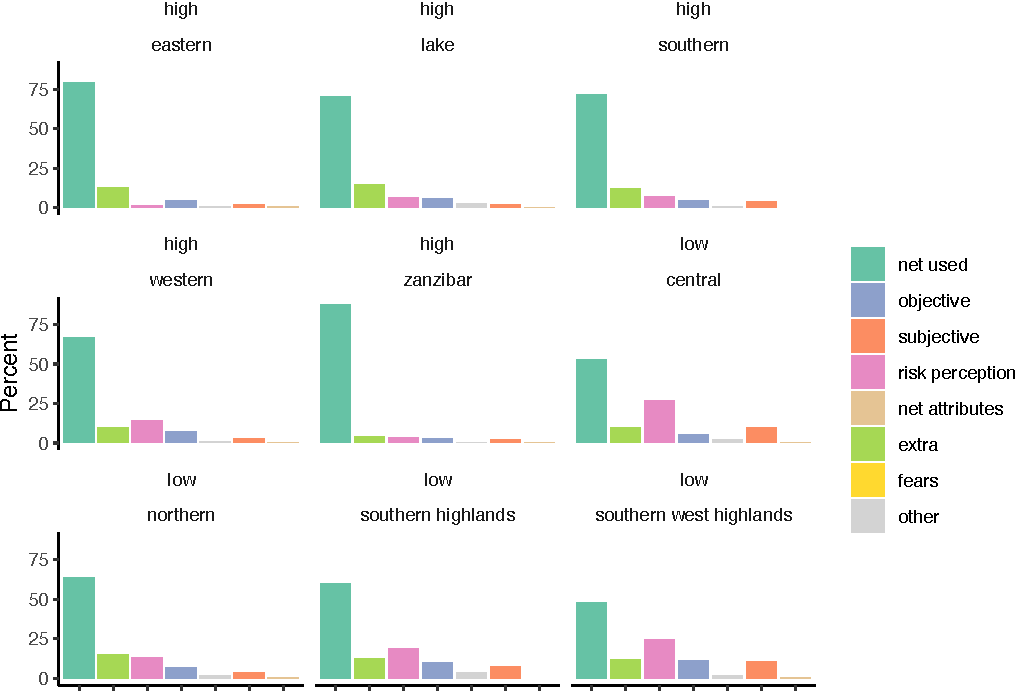
\includegraphics[width=0.8\linewidth]{reasons_paper_files/figure-latex/tz_facet-1} 

}

\caption{\label{tz_facet}Reported net use and reasons for non-use by low and high transmission zones, Tanzania 2017-18 MIS}\label{fig:tz_facet}
\end{figure}

\begin{figure}

{\centering 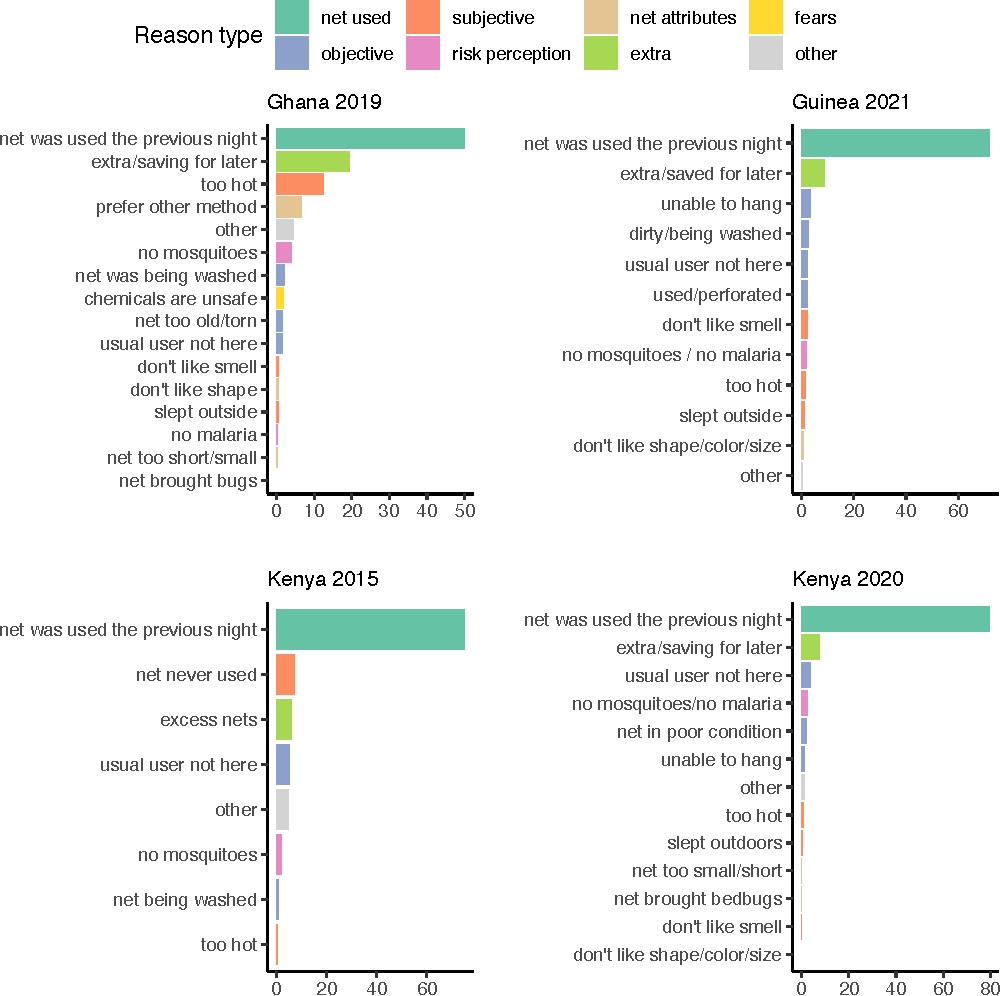
\includegraphics[width=1\linewidth]{reasons_paper_files/figure-latex/gk_reas-1} 

}

\caption{\label{gk_reas}Reasons nets were not used the previous night, Ghana, Guinea, Kenya}\label{fig:gk_reas}
\end{figure}

\begin{figure}

{\centering 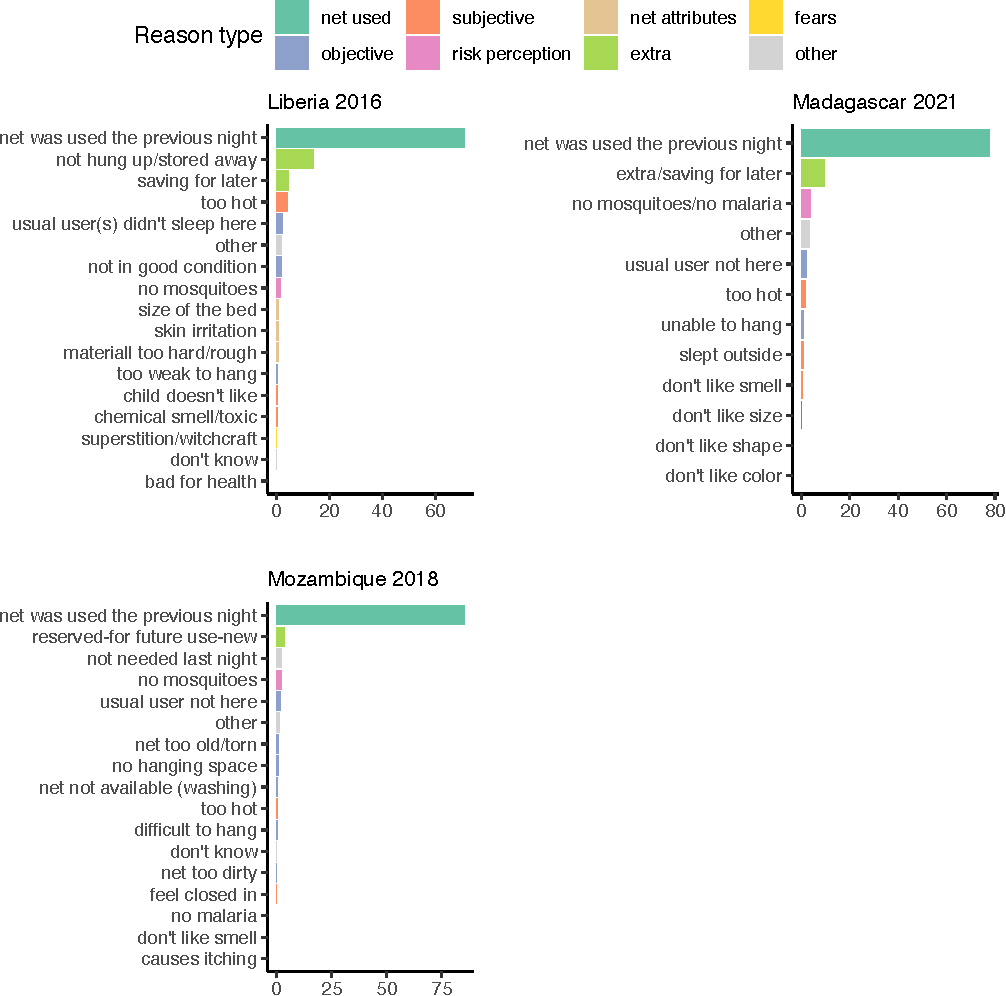
\includegraphics[width=1\linewidth]{reasons_paper_files/figure-latex/lm_reas-1} 

}

\caption{\label{lm_reas}Reasons nets were not used the previous night, Liberia, Madagascar, and Mozambique}\label{fig:lm_reas}
\end{figure}

\begin{figure}

{\centering 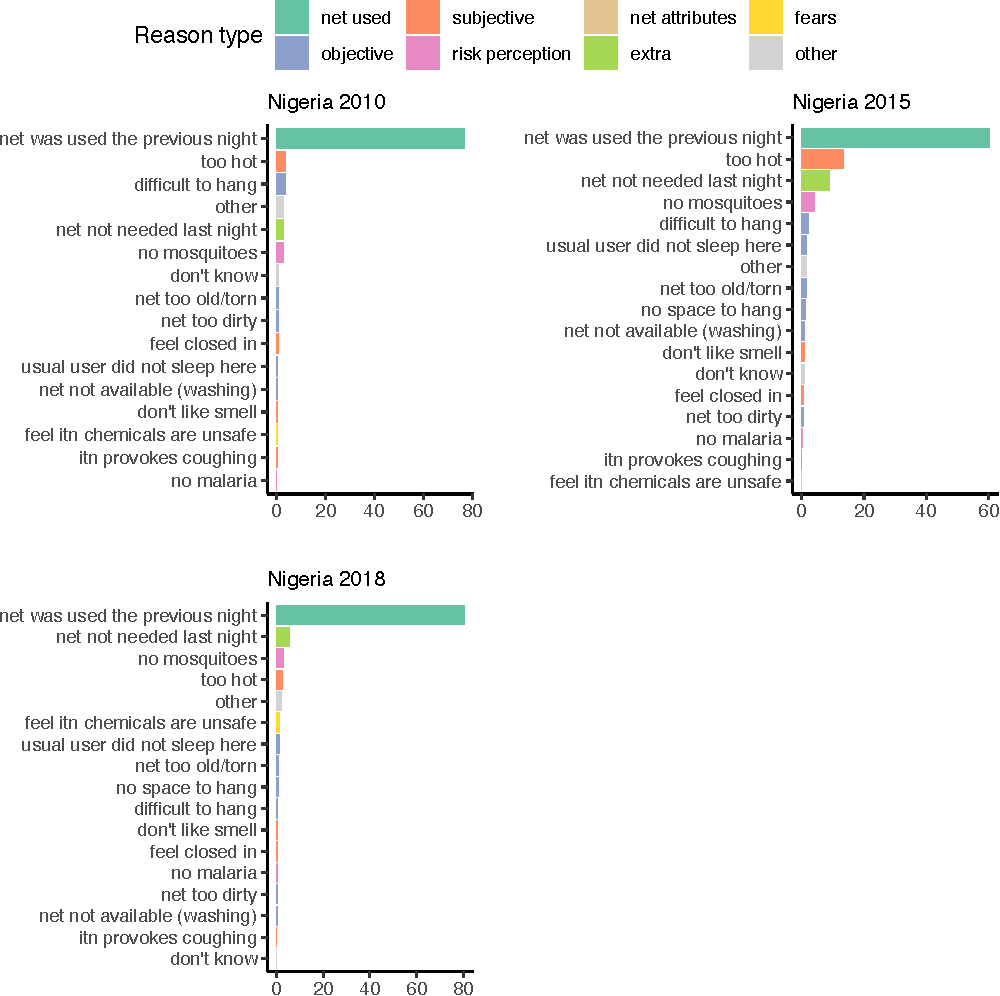
\includegraphics[width=1\linewidth]{reasons_paper_files/figure-latex/ng_reas-1} 

}

\caption{\label{ng_reas}Reasons nets were not used the previous night, Nigeria}\label{fig:ng_reas}
\end{figure}

\begin{figure}

{\centering 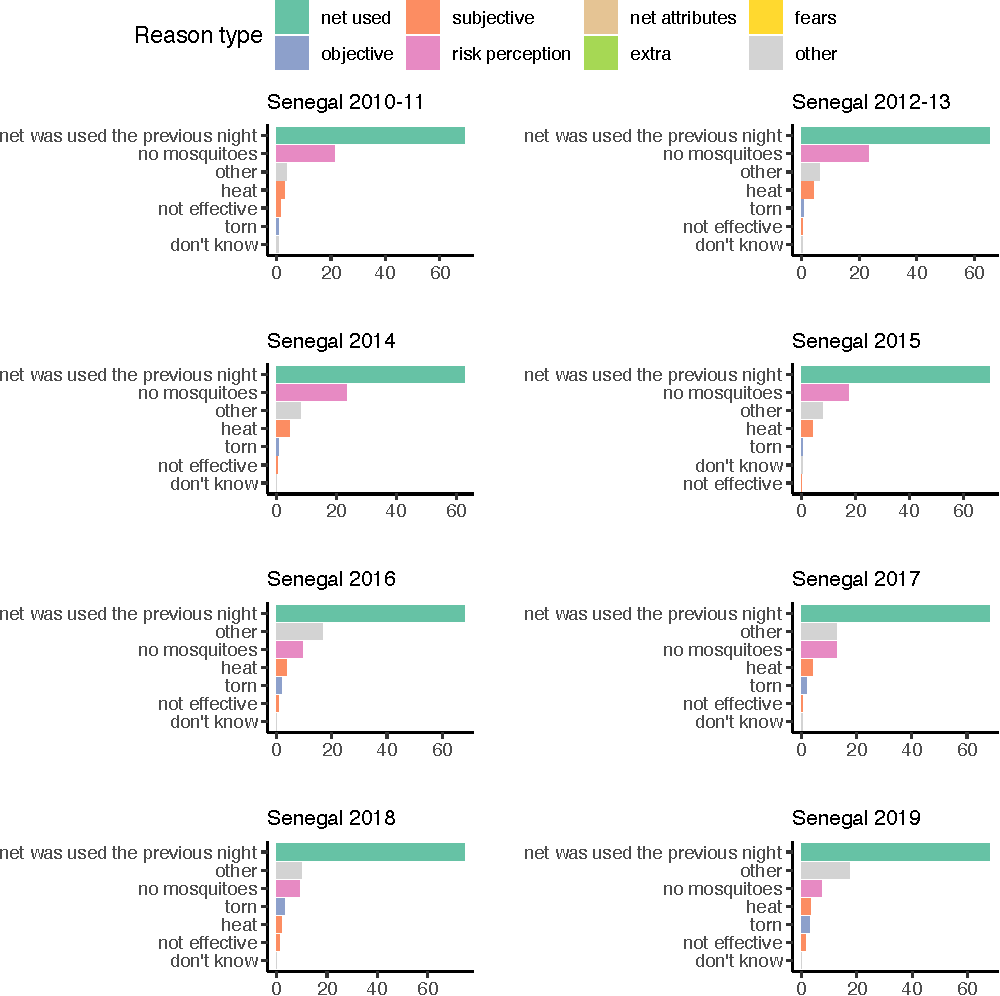
\includegraphics[width=1\linewidth]{reasons_paper_files/figure-latex/sn_reas-1} 

}

\caption{\label{sn_reas}Reasons nets were not used the previous night, Senegal}\label{fig:sn_reas}
\end{figure}

\begin{figure}

{\centering 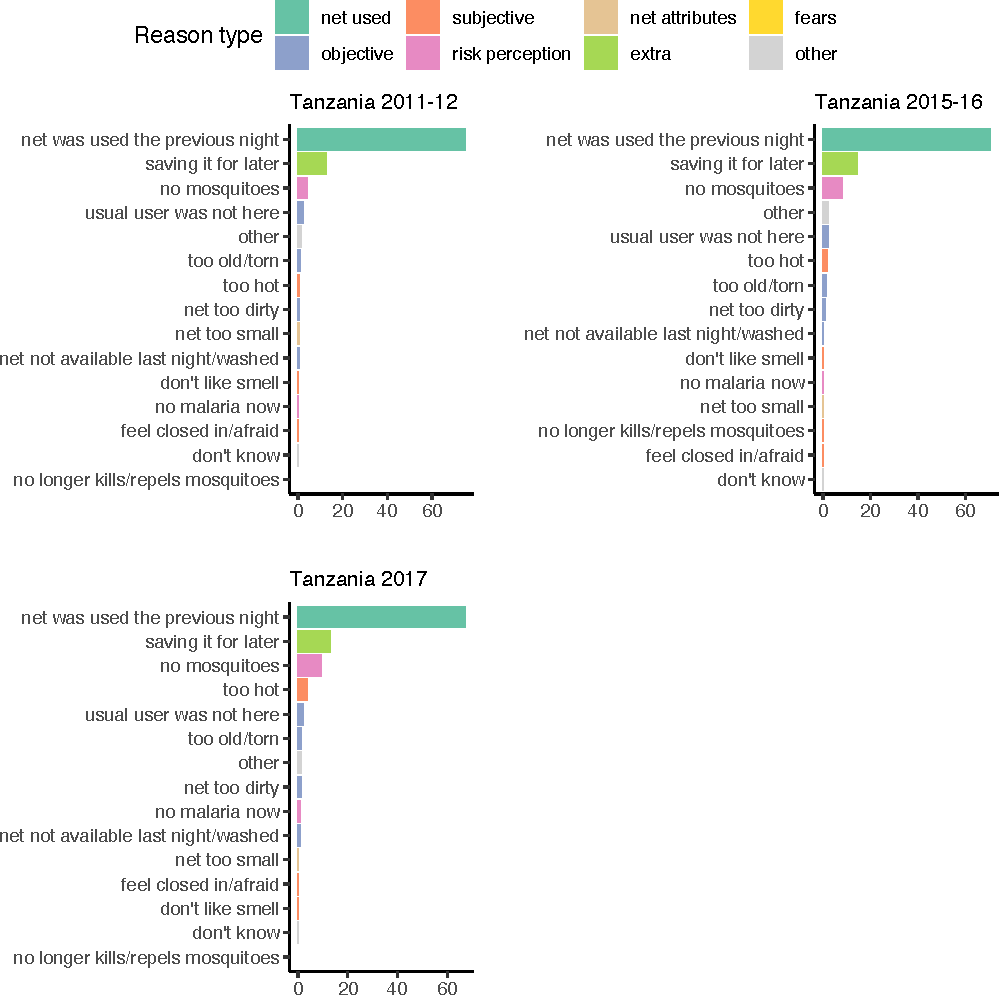
\includegraphics[width=1\linewidth]{reasons_paper_files/figure-latex/tz_reas-1} 

}

\caption{\label{tz_reas}Reasons nets were not used the previous night, Tanzania}\label{fig:tz_reas}
\end{figure}

\begin{figure}

{\centering 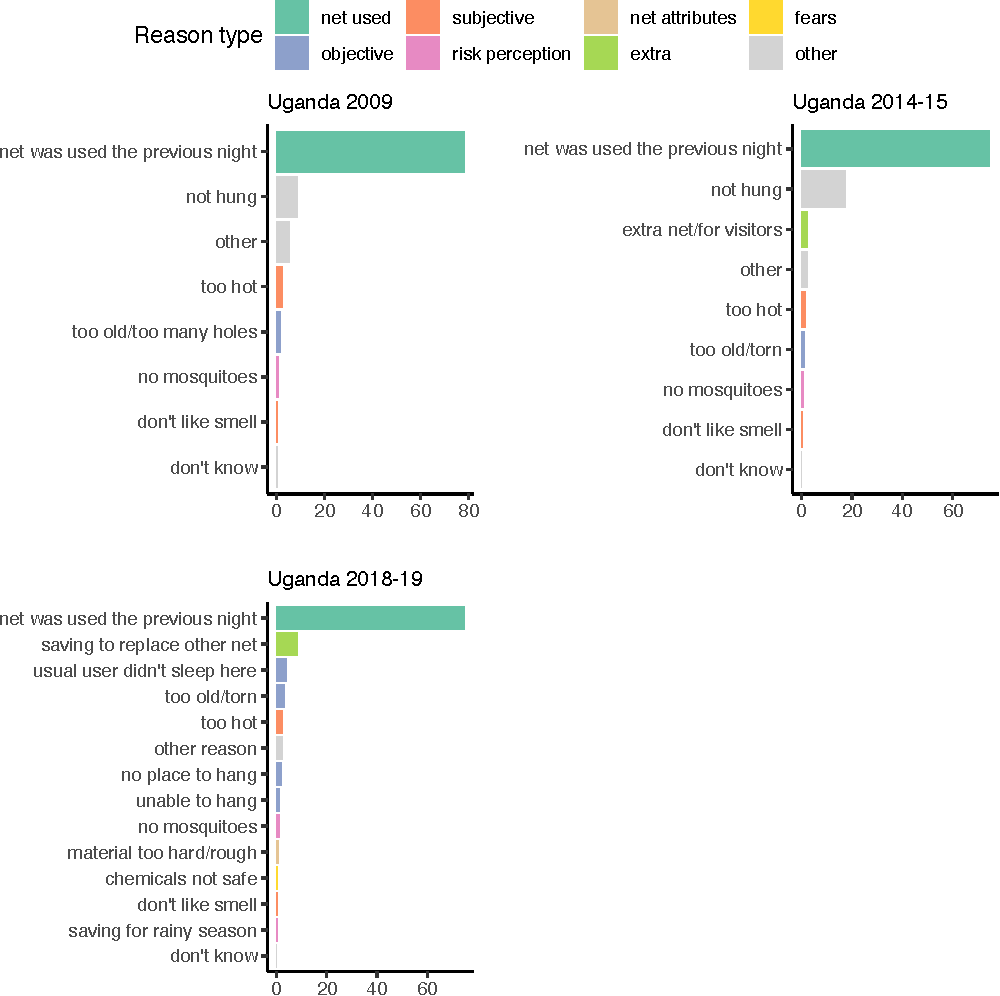
\includegraphics[width=1\linewidth]{reasons_paper_files/figure-latex/ug_reas-1} 

}

\caption{\label{ug_reas}Reasons nets were not used the previous night, Uganda}\label{fig:ug_reas}
\end{figure}

\bibliography{mybibfile.bib}


\end{document}
